% Created 2021-01-24 Sun 22:49
% Intended LaTeX compiler: pdflatex
\documentclass[11pt]{article}
\usepackage[utf8]{inputenc}
\usepackage[T1]{fontenc}
\usepackage{graphicx}
\usepackage{grffile}
\usepackage{longtable}
\usepackage{wrapfig}
\usepackage{rotating}
\usepackage[normalem]{ulem}
\usepackage{amsmath}
\usepackage{textcomp}
\usepackage{amssymb}
\usepackage{capt-of}
\usepackage{hyperref}
\usepackage{minted}
\hypersetup{colorlinks=true, linkcolor=black, filecolor=red, urlcolor=blue}
\usepackage[turkish]{babel}
\author{Eren Hatırnaz}
\date{5 Ocak 2020}
\title{Yazılım Gündemi - 2020/01\\\medskip
\large 1-5 Ocak 2020}
\hypersetup{
 pdfauthor={Eren Hatırnaz},
 pdftitle={Yazılım Gündemi - 2020/01},
 pdfkeywords={},
 pdfsubject={},
 pdfcreator={Emacs 27.1 (Org mode 9.3)},
 pdflang={Turkish}}
\begin{document}

\maketitle
\tableofcontents \clearpage\shorthandoff{=}

\begin{center}
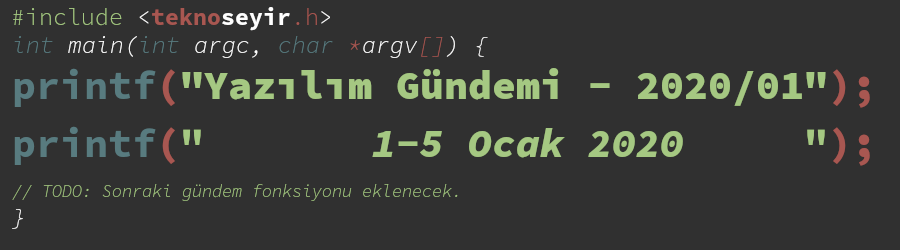
\includegraphics[width=.9\linewidth]{gorseller/yazilim-gundemi-banner.png}
\end{center}
\begin{center}
\href{../../2019/23/yazilim-gundemi-23.pdf}{< Önceki Gündem} | \textbf{1-5 Ocak 2020} | \href{../02/yazilim-gundemi-2020-02.pdf}{Sonraki Gündem >}

\href{https://teknoseyir.com/blog/yazilim-gundemi-2020-01}{TeknoSeyir'de Oku}
\end{center}

\section{Rust dilinin 32-bit Apple sistemler için \href{https://blog.rust-lang.org/2020/01/03/reducing-support-for-32-bit-apple-targets.html}{desteği azalıyor}}
\label{sec:org9d79a23}
\href{https://www.rust-lang.org/}{Rust}, gün geçtikçe popülerliği daha da artan bir programlama dili. Yazılım
gündemi yazıları yazmaya başladığımdan beri bunu daha iyi görüyorum. Hemen her
hafta Rust ile ilgili bir gelişme oluyor, olmazsa bile geliştiricilerin
ilgileri gitgide artıyor. Bununla birlikte Rust'ın geliştirilme süreci de hızla
devam ediyor. Bir önceki yazılım gündeminde Rust programlama dilinin 1.41.0
sürümünün yayınlandığını duyurmuştum. Bu hafta ise bloglarında yayınlandıkları
bir yazı ile 1.42.0 sürümü itibariyle, 32-bit Apple sistemler için Rust
programlama dilinin desteğinin azaltıldığını açıkladılar ve bu platformun
destek sürecini Tier 3 ismini verdikleri kategoriye taşıdılar.

Rust geliştirici takımının çeşitli platformlardaki destek süreçlerini
tanımladıkları şöyle bir dokümanları mevcut: \href{https://forge.rust-lang.org/release/platform-support.html}{Platform Support}. Bu dokümana göre
üç destek grubu var. Bunlar şu şekilde:

\begin{itemize}
\item Tier 1: Bu kategorideki platformlarda Rust'ın \uline{çalışması garanti} edilmiştir.
\item Tier 2: Rust'ın \uline{derlenmesinin garanti} edildiği platformlar listesidir.
\item Tier 2.5: Yine Rust'ın derlenmesinin garanti edildiği platformlar fakat bu
listedeki platformlar için \texttt{rustup} aracı ile güncelleme özelliği desteği
sağlanmıyor. Kaynak kodlarını kullanarak kendiniz derlemeniz gerekiyor.
\item Tier 3: \uline{Hiçbir garantinin verilmediği} platformlar listesi. Rust dilini
kaynak kodları kullanarak bu sistemlerde derlemeye çalışabilirsiniz fakat
hatalarla veya eksik özelliklerle karşılaşmanız çok mümkün.
\end{itemize}

İşte 32-bit Apple sistemler de 1.42.0 sürümüyle birlikte Tier 3 kategorisinde
altında yer alacak. Bu kategori değişikliğinden etkilenen platformların kod
isimleri ise bu şekilde:

\begin{itemize}
\item armv7-apple-ios
\item armv7s-apple-ios
\item i386-apple-ios
\end{itemize}

32-bit sistemlere desteğin kesilmesi günümüzde çok şaşırmadığımız bir durum
elbette fakat yine de desteğin neden kesildiğini açıklamakta fayda var. Rust
takımından önce zaten Apple \href{https://support.apple.com/en-us/HT208436}{macOS 10.15} ve \href{https://developer.apple.com/documentation/uikit/app\_and\_environment/updating\_your\_app\_from\_32-bit\_to\_64-bit\_architecture}{iOS 11} ile birlikte 32-bit desteğini
sonlandırmıştı, üstelik Xcode ile 32-bit derleme yapmanın da önüne geçmişti.
Zaten günümüzde 32-bit sistem ile geliştirme yapmak pek de mümkün olmadığı için
Rust takımı da böyle bir varar vermiş ve bence de yerinde bir karar.
\section{Oracle, Amazon API'sini kopyalamakla \href{https://arstechnica.com/tech-policy/2020/01/oracle-copied-amazons-api-was-that-copyright-infringement/}{suçlanıyor}}
\label{sec:org6fbfffb}
Oracle ve Google arasında Java API'si (Application Programming Interface)
üzerinden devam etmekte olan hukuk savaşını zaten yıllardır Haftalık Gündem
Değerlendirmesi'nde dinliyoruz. Bilmeyenler için kısaca özetlemek gerekirse
Google'ın Android işletim sistemini geliştirirken Java API'sini birebir
kopyaladığını ve telif haklarını ihlal ettiğini söyleyen Oracle, Google'ın
cezalandırılmasını istiyor. Burada kopyalamaktan kasıt kopyala\&yapıştır
kullanımındaki gibi değil. Google, Java'nın API sistemindeki fonksiyonellikleri
ve method isimlerinin aynısını kullanarak bir nevi Java'yı yeniden yazmasından
bahsediyoruz.

Bu hafta ArsTechnina sitesinde çıkan yazıda ise Oracle şirketinin Amazon'un S3
isimli veri depolama hizmetinin API sistemini kopyaladığı iddiası var. Hatta
sadece iddia da değil, Oracle Cloud hizmetinin dokümantasyonundaki şu sayfa
doğrudan bunu ortaya çıkıyor: \href{https://docs.cloud.oracle.com/iaas/Content/Object/Tasks/s3compatibleapi.htm}{Amazon S3 Compatibility API}. E hal böyleyken
demezler mi adama "bu ne perhiz, bu ne lahana turşusu?" diye, işte ArsTechnica
da tam olarak bunu söylemiş.

Bu tarz API "kopyalamaları" her ne kadar üzerine tartışılabilir konular olsa da
biraz gerekli olduğunu düşünüyorum. Amazon S3 örneğinden gidecek olursak,
Amazon bulut bilişim sektöründe çok büyük bir oyuncu ve bu oyuncuyla rekabet
edebilmek için onunla hemen hemen aynı özellikleri sunmak gerekiyor. Bunu
yaparken de API sistemi ne kadar Amazon'unkine benzerse geliştiriciler de o
kadar az efor sarf ederek Amazon ekosisteminden çıkabilirler. Yani minumum kod
değişikliği ile bu dönüşümün sağlanması rekabet ortamı için önemli bir konu.

Bu konuda siz ne düşünüyorsunuz? Bu tarz API benzerliklerinin sağlanması sizce
büyük firmalarla rekabet edilebilmesi için gerekli mi yoksa ne olursa olsun
firma özgün bir çözüm mü sunmalı? Yorumlar bölümünde konuşalım.
\section{Amerika yapay zeka yazılımlarının ihracına \href{https://www.reuters.com/article/us-usa-artificial-intelligence/u-s-government-limits-exports-of-artificial-intelligence-software-idUSKBN1Z21PT}{sınırlama getiriyor}}
\label{sec:org53861a3}
Yapay zeka yazılımları üreten Amerika merkezli şirketler Pazartesi gününden
itibaren yazılımlarını Kanada harici, deniz aşırı ülkelere ihraç ederken bir
lisans almak zorunda kalacaklar. Yeni ihracat tedbiri özellikle coğrafi
görüntüleme yazılımlarını ilgilendirmekle birlikte askeri ya da sivil amaçlarla
olsun fark etmeksizin herhangi bir hedef belirleme süreci içeren yazılımları ve
donanımları da kapsamakta.
\section{Yaklaşan Etkinlikler}
\label{sec:orga8af200}
\begin{longtable}{|p{8cm}|l|l|}
\hline
Etkinlik İsmi & Yeri & Tarihi\\
\hline
\endfirsthead
\multicolumn{3}{l}{Önceki sayfadan devam ediyor} \\
\hline

Etkinlik İsmi & Yeri & Tarihi \\

\hline
\endhead
\hline\multicolumn{3}{r}{Devamı sonraki sayfada} \\
\endfoot
\endlastfoot
\hline
\href{https://www.meetup.com/IBMCloudTR/events/267424987/}{Online Webinar: Text Analysis Application on Kubernetes} & Online & 6 Ocak 13:00\\
\href{https://www.meetup.com/IBMCloudTR/events/267577304/}{Analyze Real Time Bank Customer Data} & İstanbul & 9 Ocak 19:00\\
\href{https://www.meetup.com/trendyol/events/267060271/}{Domain Driven Design} & İstanbul & 9 Ocak 20:30\\
\href{https://www.meetup.com/Agile-Bulusmalar/events/267522502/}{Agile Talks 2020 Episode 1} & İstanbul & 11 Ocak 11:00\\
\href{https://www.eventbrite.com/e/busiber-siber-ks-kamp-2020-registration-85540641361}{BÜSİBER Siber Kış Kampı 2020} & İstanbul & 13 Ocak 09:00\\
\href{https://kommunity.com/frontend-istanbul/events/the-future-of-react-server-rendering-is-not-a-silver-bullet}{The Future of React \& Server Rendering is not a Silver Bullet} & İstanbul & 16 Ocak 19:30\\
\hline
\end{longtable}

\textbf{\textbf{\href{https://kamp.siberkulupler.com/}{Siber Küme Kış Kampı} başvuruları başladı. Son başvuru tarihi 10 Ocak.}}
\section{Diğer Haberler}
\label{sec:orga0a2d67}
\begin{itemize}
\item Rust dilinin uzay çalışmalarındaki kullanım alanlarını araştıracak \href{https://www.reddit.com/r/rust/comments/ejdv7w/announcing\_aerorust\_the\_unofficial\_working\_group/}{çalışma
grubu kuruldu}: \href{https://github.com/AeroRust/Welcome}{AeroRust}, \href{https://github.com/AeroRust/awesome-space}{Faydalı Kaynaklar}.
\item .NET Teknolojileri ile platformlar-arası (cross-platform) uygulama geliştirme
kütüphanesi Uno Platform, \href{https://platform.uno/uno-platform-2-0-reloaded-general-availability-hot-reload-and-more/}{2.0 sürümünü duyurdu}, \href{https://github.com/unoplatform/uno}{GitHub Deposu}.
\item Android Emulator \href{https://androidstudio.googleblog.com/2020/01/emulator-2934-canary.html}{29.3.4 Canary sürümü yayınlandı}.
\item Python için iş kuyrukları oluşturma kütüphanesi RQ, \href{https://github.com/rq/rq/releases/tag/v1.2.0}{1.2.0 sürümünü yayınladı}.
\item Popüler PHP HTTP istemcilerinden Guzzle, \href{https://github.com/guzzle/guzzle/releases/tag/7.0.0-beta.1}{7.0.0-beta.1 sürümünü yayınladı}.
\item Postman alternatifi olan Milkman, \href{https://github.com/warmuuh/milkman/releases/tag/4.0.0}{4.0.0 sürümünü yayınladı}.
\end{itemize}
\section{Lisans}
\label{sec:org32d118a}
\begin{center}
\begin{center}

\includegraphics[height=1.5cm]{../../../img/CC_BY-NC-SA_4.0.png}
\end{center}

\href{yazilim-gundemi-2020-01.pdf}{Yazılım Gündemi - 2020/01} yazısı \href{https://erenhatirnaz.github.io}{Eren Hatırnaz} tarafından \href{http://creativecommons.org/licenses/by-nc-sa/4.0/}{Creative Commons
Atıf-GayriTicari-AynıLisanslaPaylaş 4.0 Uluslararası Lisansı} (CC BY-NC-SA 4.0)
ile lisanslanmıştır.
\end{center}
\end{document}
